\section{eo\-Gen\-Op$<$ EOT $>$ Class Template Reference}
\label{classeo_gen_op}\index{eoGenOp@{eoGenOp}}
The base class for General Operators Subclass this operator is you want to define an operator that falls outside of the {\bf eo\-Mon\-Op}{\rm (p.\,\pageref{classeo_mon_op})}, {\bf eo\-Bin\-Op}{\rm (p.\,\pageref{classeo_bin_op})}, {\bf eo\-Quad\-Op}{\rm (p.\,\pageref{classeo_quad_op})} classification.  


{\tt \#include $<$eo\-Gen\-Op.h$>$}

Inheritance diagram for eo\-Gen\-Op$<$ EOT $>$::\begin{figure}[H]
\begin{center}
\leavevmode
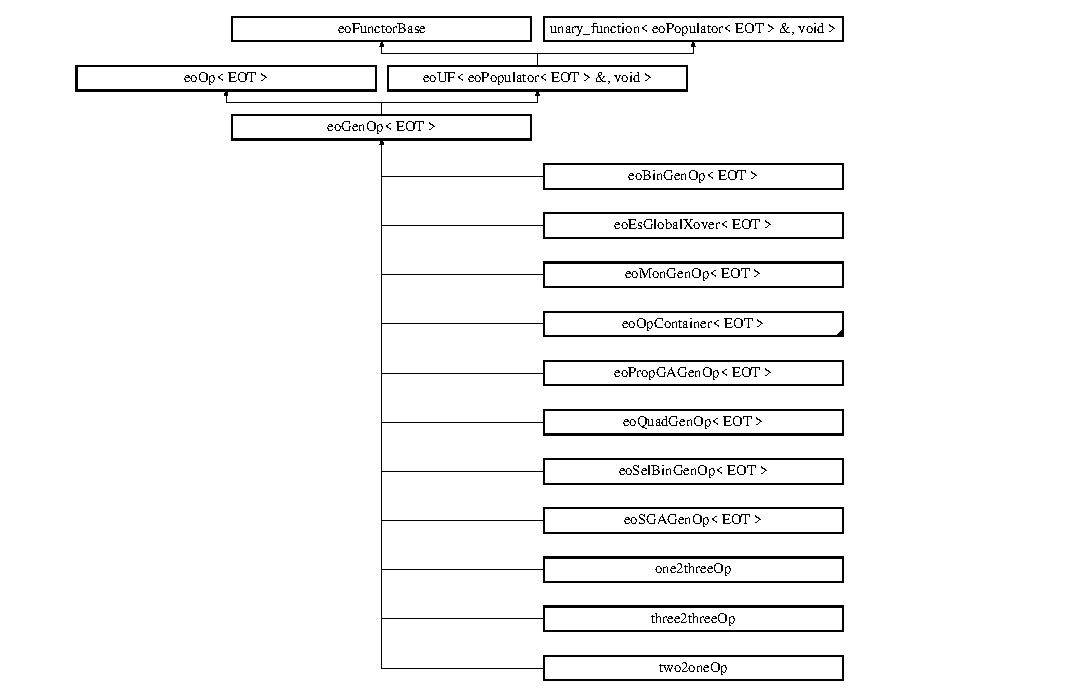
\includegraphics[height=8.91923cm]{classeo_gen_op}
\end{center}
\end{figure}
\subsection*{Public Member Functions}
\begin{CompactItemize}
\item 
{\bf eo\-Gen\-Op} ()\label{classeo_gen_op_a0}

\begin{CompactList}\small\item\em Ctor that honors its superclass. \item\end{CompactList}\item 
virtual unsigned {\bf max\_\-production} (void)=0\label{classeo_gen_op_a1}

\begin{CompactList}\small\item\em Max production is used to reserve space for all elements that are used by the operator, not setting it properly can result in a crash. \item\end{CompactList}\item 
virtual std::string {\bf class\-Name} () const =0\label{classeo_gen_op_a2}

\item 
void {\bf operator()} ({\bf eo\-Populator}$<$ {\bf EOT} $>$ \&\_\-pop)\label{classeo_gen_op_a3}

\begin{CompactList}\small\item\em The pure virtual function that needs to be implemented by the subclass. \item\end{CompactList}\end{CompactItemize}
\subsection*{Protected Member Functions}
\begin{CompactItemize}
\item 
virtual void {\bf apply} ({\bf eo\-Populator}$<$ {\bf EOT} $>$ \&\_\-pop)=0\label{classeo_gen_op_b0}

\begin{CompactList}\small\item\em the function that will do the work \item\end{CompactList}\end{CompactItemize}


\subsection{Detailed Description}
\subsubsection*{template$<$class EOT$>$ class eo\-Gen\-Op$<$ EOT $>$}

The base class for General Operators Subclass this operator is you want to define an operator that falls outside of the {\bf eo\-Mon\-Op}{\rm (p.\,\pageref{classeo_mon_op})}, {\bf eo\-Bin\-Op}{\rm (p.\,\pageref{classeo_bin_op})}, {\bf eo\-Quad\-Op}{\rm (p.\,\pageref{classeo_quad_op})} classification. 

The argument the operator will receive is an {\bf eo\-Populator}{\rm (p.\,\pageref{classeo_populator})}, which is a wrapper around the original population, is an instantiation of the next population and has often a selection function embedded in it to select new individuals.

Note that the actual work is performed in the apply function. AND that the apply function is responsible for invalidating the object if necessary 



Definition at line 57 of file eo\-Gen\-Op.h.

The documentation for this class was generated from the following file:\begin{CompactItemize}
\item 
eo\-Gen\-Op.h\end{CompactItemize}
